\chapter{\label{chapter:Propagators}GMAT's Propagators}
\chapauthor{Darrel J. Conway}{Thinking Systems, Inc.}

Chapter~\ref{chapter:PropagatorStates} describes the classes used to represent the state of the
objects in a Mission Control Sequence, but does not define the pieces that perform the time
evolution for that state.  Those components -- the propagators -- are described in this chapter.

\section{The Propagator Classes}

The components that are instrumental in time evolution are shown in
Figure~\ref{figure:PropagatorClasses}.

\begin{figure}[htb]
\begin{center}
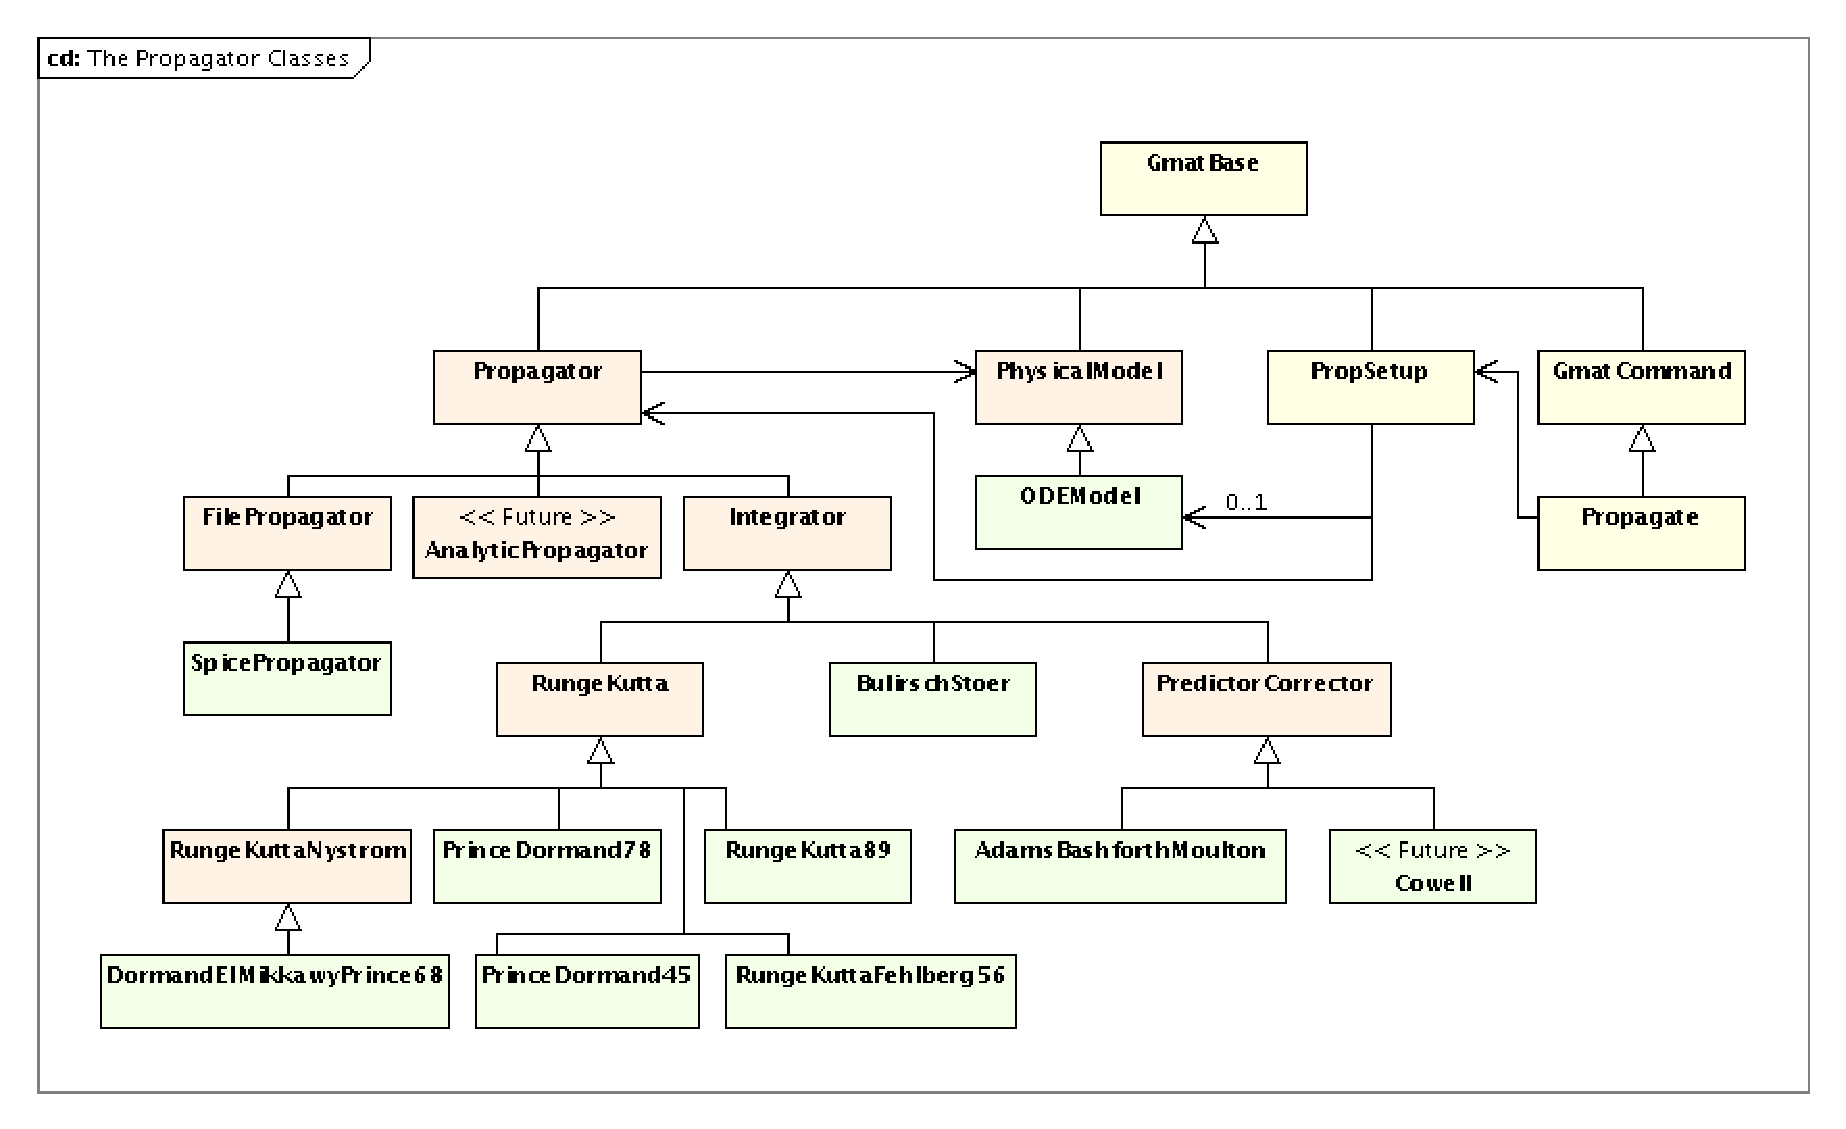
\includegraphics[scale=0.5]{Images/ThePropagatorClasses.eps}
\caption[Classes Used to Propagate State Data]{\label{figure:PropagatorClasses}Classes Used
to Propagate State Data.  Base classes are shown in orange.  Classes that instantiate the objects
used in numerical integration are in green.  Analytic propagation elements are in blue.  Classes
that are used to drive the propagation process, and other base level classes, are shown in yellow.}
\end{center}
\end{figure}

The numerical integration portion of the propagation system, shown in green in the figure, consists
of a differential equation model and numerical integrator paired to perform the precision
integration. The ODEModel class is a container class that accumulates all of the differential
equation data modeled in the mission, and reports the resulting changes in the elements of the
state vector. Details of the force model components of the differential equation model are described
in Chapter~\ref{chapter:ForceModel}.  Other differential equation models are described separately.

\section{The Propagator Base Class}

\subsection{Class Attributes}

\begin{itemize}
\item \textbf{PropVector *thePropVector}
\end{itemize}

\subsection{Class Methods}

\begin{itemize}
\item \textbf{bool Initialize()}
\end{itemize}

\section{Numerical Integration}


\subsection{\label{section:TheODEModel} The Derivative Models}

\begin{figure}[htb]
\begin{center}
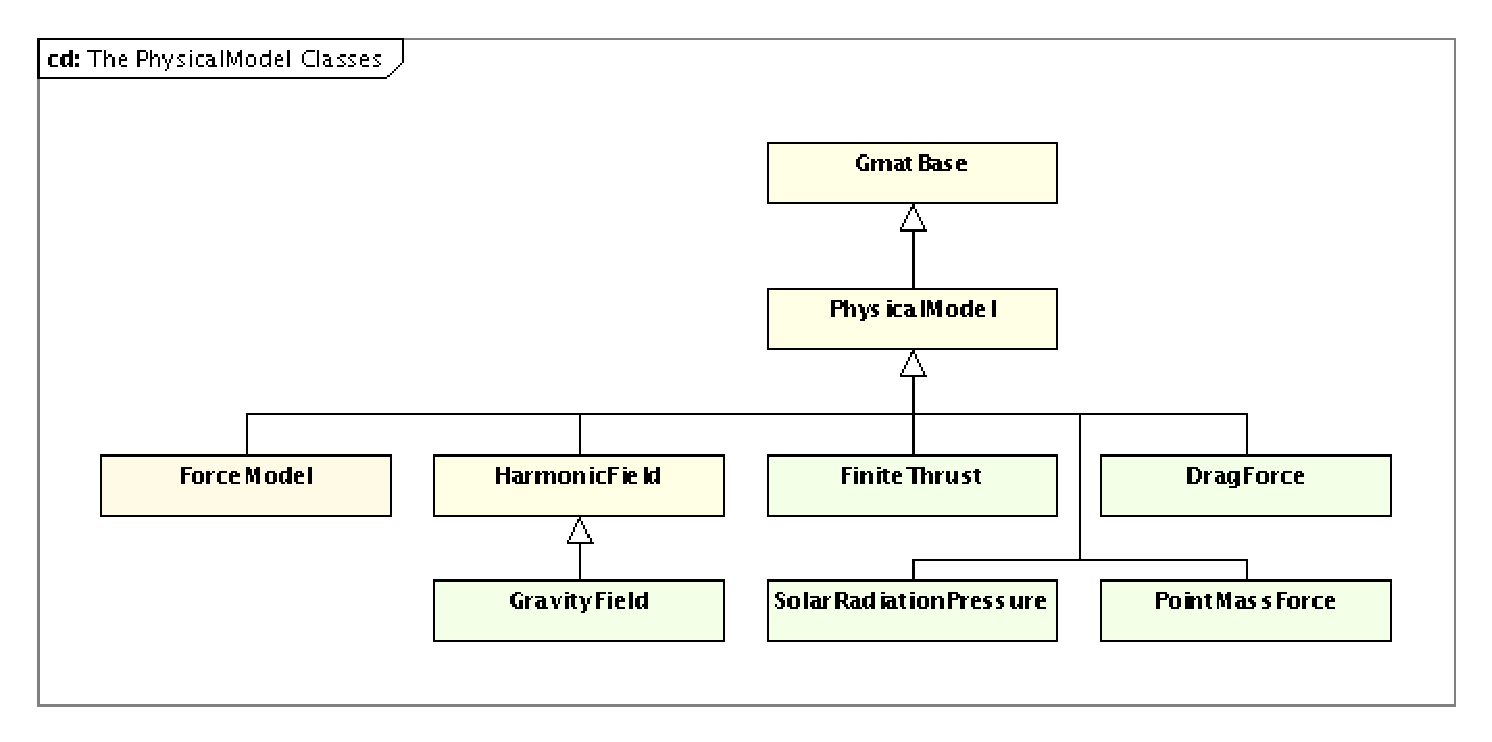
\includegraphics[scale=0.5]{Images/ThePhysicalModelClasses.eps}
\caption[The Derivative Model Classes]{\label{figure:PhysicalModelClasses}The Derivative Model
Classes.  This figure shows the classes used to provide derivative information to GMAT's
integrators.}
\end{center}
\end{figure}

\subsection{Initialization of the Derivative Model}


\begin{figure}[htb]
\begin{center}
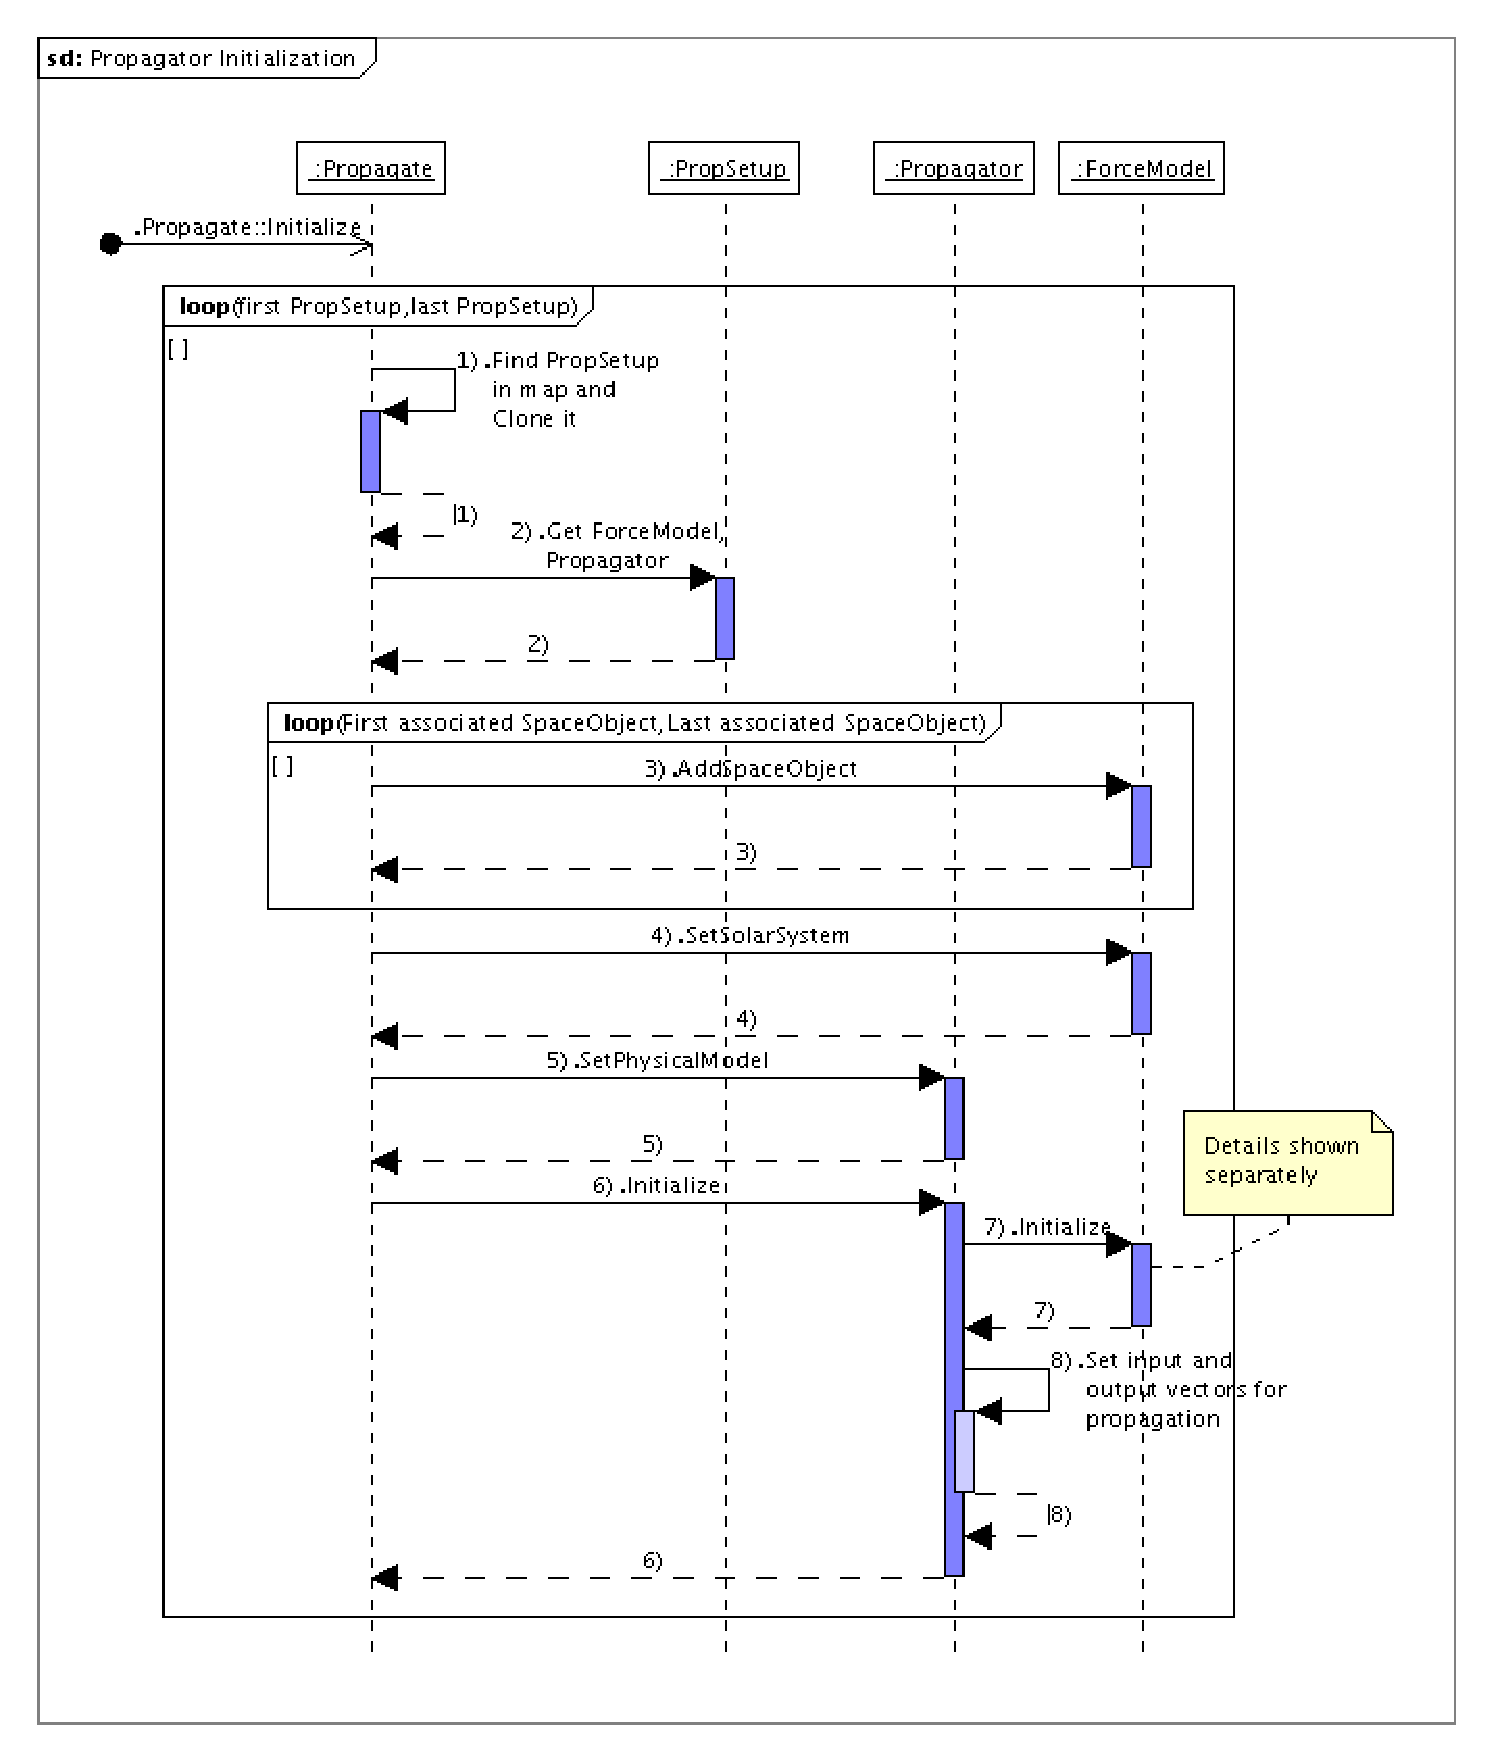
\includegraphics[scale=0.5]{Images/PropagatorInitialization.eps}
\caption[Propagator Initialization]{\label{figure:PropagatorInitialization}Propagator
Initialization.  This sequence diagram shows the process used to prepare a propagator for use in
the Mission Control Sequence.}
\end{center}
\end{figure}


\begin{figure}[htb]
\begin{center}
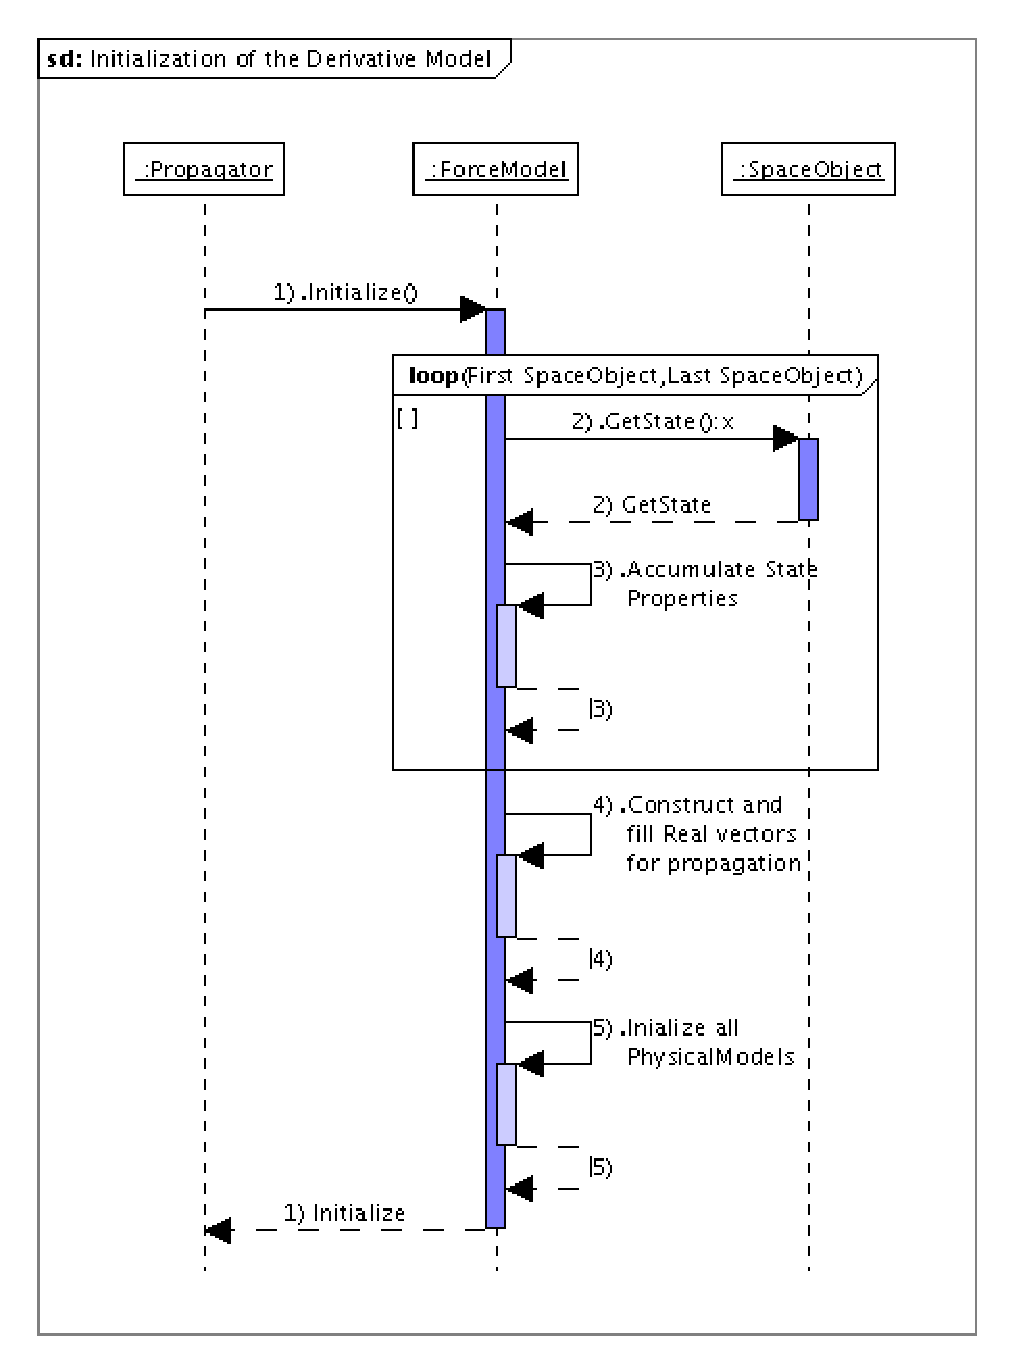
\includegraphics[scale=0.5]{Images/InitializationoftheDerivativeModel.eps}
\caption[Derivative Model Initialization]{\label{figure:DerivativeModelInitialization}Derivative
Model Initialization.  This sequence diagram shows the process used to build the data that is
numerically integrated during propagation.}
\end{center}
\end{figure}


\subsection{Finalizing Initialization: The PrepareToPropagate() Method}

\begin{figure}[htb]
\begin{center}
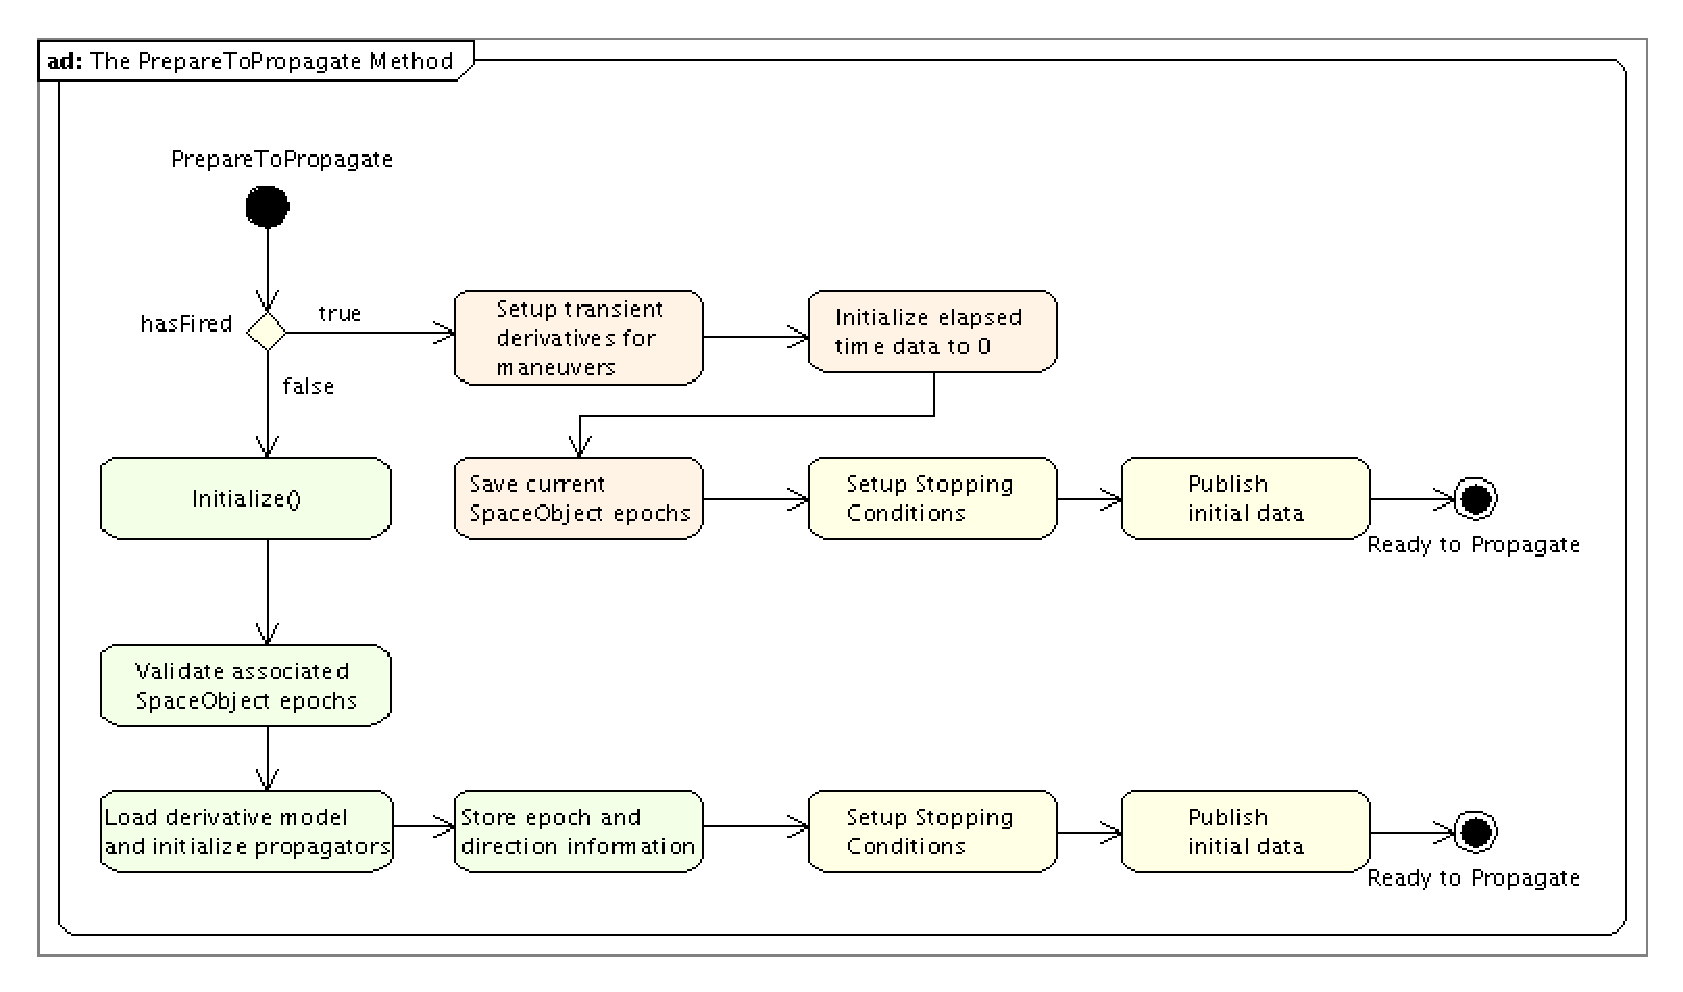
\includegraphics[scale=0.5]{Images/ThePrepareToPropagateMethod.eps}
\caption[Final Propagator Initialization:PrepareToPropagate())]
{\label{figure:PrepareToPropagate}Final Propagator Initialization:
PrepareToPropagate()}
\end{center}
\end{figure}


\subsection{Propagation}



\subsection{Completing Propagation}


\section{Analytic Propagation}

\section{File Based Propagation}

\section{Propagation Examples}

\subsection{\label{section:IntegratorExample}A Numerical Integration Example}

\subsection{\label{section:SpiceExample}A SPICE File Propagation Example}

\subsection{\label{section:MixedModePropagation}A Mixed Mode Example}

